% !TEX encoding = UTF-8 Unicode
% Capítulo 2 - Nociones preliminares
\chapter[Nociones preliminares]{Nociones preliminares}
\label{chap:2}

En este capítulo introduciremos las definiciones y conceptos básicos con los que se trabajará durante el desarrollo de 
esta tesina. Se presentarán la \textit{minería de procesos} (\autoref{sec:2.process mining}), 
las \textit{redes de Petri} (\autoref{sec:2.Petrinets}), \textit{Vectores Parikh} (\autoref{sec:2.parikh}), 
\textit{Dominios numéricos abstractos} y su aplicación al desubrimiento de procesos (\autoref{sec:2.discovery}).
Luego se realizará una introducción a \textit{satifabilidad módulo teorías} 
y se introducirán los conceptos utilizados de \textit{logs} (\autoref{sec:2.logs}) 
e \textit{información negativa} (\autoref{sec:2.negative}).

Por último, utilizando estos conceptos, plantearemos de manera concreta el problema a resolver en 
esta tesina (\autoref{sec:2.problem}).

\section{Minería de procesos} 
\label{sec:2.process mining}

La minería de procesos es el nombre dado a un conjunto de técnicas que tienen
como objetivo extraer información referente al proceso de un cierto sistema
con el objetivo de poder analizar, probar ciertas propiedades 
así como implementar posibles mejoras sobre dicho proceso.

A diferencia de las técnicas clásicos de las técnicas de minería de datos, el foco
está en los procesos, en el flujo de un sistema.

\subsection{Logs} 
\label{sec:2.logs}

La minería de procesos tiene su punto inicial en la recopilación de un \textit{log de eventos}. 
Un evento refiere a la ocurrencia de una actividad de un sistema $\sys$ y
una traza de eventos -o simplemente traza- se define como una sucesión
ordenada de estos eventos, por lo general, generadas de manera automática.
Un log de eventos -o simplemente \textit{log}- por su parte, se conforma de un
conjunto de trazas cada una de las cuales corresponden a una instancia única 
de la ejecución de $\sys$, llamada, instancia de proceso o caso.
Durante la minería de procesos, suelen utilizarse varios casos sobre un mismo proceso~\cite{Aalst2004}.

Un log posee los siguientes elementos constitutivos fundamentales: un conjunto de actividades,
un cierto orden temporal en el cual ocurren y una etiqueta del  caso o instancia de proceso
que agrupe dichas actividades en trazas.
Sin embargo, un log puede contener, además, datos adicionales que, aunque no sean fundamentales, pueden
ayudar a la minería de procesos otorgándole mayor nivel de detalle y claridad.

La \autoref{tab:log_ex} muestra un ejemplo parcial de un conjunto de logs con información 
adicional (e.g. medio, tipo, user) que permite un entendimiento mayor del devenir del proceso.

\begin{table}[t]
\tiny

\def\sep{\hspace{10pt}}
\begin{tabular}{r   c   l   l   r   c   c}
  \tiny \#Caso
& \tiny Timestamp
& \tiny Medio
& \tiny Tipo
& \tiny Urgencia
& \tiny Usr
& \tiny Grupo
\\
\midrule
 970 & 2015-12-31 23:55:12 & Teléfono & Aviso & 0 & Andrés & Nivel 1\newrow
 970 & 2015-12-31 23:56:22 & Mail & Reclamo & 0 & Andrés & Nivel 1\newrow
 970 & 2016-01-01 00:05:11 & Teléfono & Reclamo & 1 & Andrés & Nivel 1\newrow
 971 & 2016-01-01 00:30:44 & Mail & Abierto & 2 & Gonzalo & Nivel 1\newrow
 971 & 2016-01-01 00:30:44 & Mail & Resuelto & 2 & Gonzalo & Nivel 1\newrow
 970 & 2016-01-01 00:30:44 & Teléfono & Derivado & 0 & Andrés & Nivel 2\newrow
 312 & 2016-01-01 15:30:01 & Mail & En progr. & 3 & Gonzalo & Nivel 3\newrow
 42 & 2016-05-04 00:00:01 & Mail & Resuelto & 10 & Lucio & Nivel x\newrow
 42 & 2016-05-04 00:00:01 & Mail & Resuelto & 10 & Lucio & Nivel x\newrow
 $\vdots$ & $\vdots$ & $\vdots$ & $\vdots$ & $\vdots$ & $\vdots$ & $\vdots$ \newrow
\end{tabular}
\vspace{0pt}
\caption{\tiny Un ejemplo artificial de un log de eventos con información adicional.}
\label{tab:log_ex}
\end{table} 


Existen diferentes formas en las que se puede representar un log y debido a que provienen de diferentes
sistemas, su representación dista de ser homogénea. Para intentar evitar esta heterogeneidad de representación,
se utiliza mayoritariamente el estándar para describir logs llamado 
\textit{e\textbf{X}tensible \textbf{E}vent \textbf{S}tream}, \textbf{XES}.

XES consiste en un lenguaje basado en XML creado específicamente para representar logs de eventos que busca 
un formato universal que permita la creación de herramientas reutilizables y la comunicación e intercambio de 
información y, aunque su objetivo primario es la minería de procesos, también se 
utiliza en otras áreas como minería de datos y análisis estadístico.
En la \autoref{fig:xeslog}, se transcribe un ejemplo artificial de un log siguiendo el estándar XES.

\begin{figure}[h]
    \begin{minted}[
    bgcolor=bg,
    frame=lines,
    framesep=2mm,
    baselinestretch=1.2,
    fontsize=\tiny]{xml}
    
  <?xml version="1.0" encoding="UTF-8" ?>
  <log xes.version="1.0">
  	<trace>
  		<string key="concept:name" value="1"/>
  		<event>
  			<string key="concept:name" value="register request"/>
  			<date key="time:timestamp" value="2010-12-30 11:02:00"/>
  			<string key="Activity" value="register request"/>
  			<string key="Costs" value="50"/>
  		</event>
  		<event>
  			<string key="concept:name" value="examine thoroughly"/>
  			<date key="time:timestamp" value="2010-12-31 10:06:00"/>
  			<string key="Activity" value="examine thoroughly"/>
  			<string key="Costs" value="400"/>
  		</event>
  	</trace>
  	<trace>
  		<string key="concept:name" value="4"/>
  		<event>
  			<string key="concept:name" value="register request"/>
  			<date key="time:timestamp" value="2011-01-06 15:02:00"/>
  			<string key="Activity" value="register request"/>
  			<string key="Costs" value="50"/>
  		</event>
  		<event>
  			<string key="concept:name" value="check ticket"/>
  			<date key="time:timestamp" value="2011-01-07 12:06:00"/>
  			<string key="Activity" value="check ticket"/>
  			<string key="Costs" value="100"/>
  		</event>
  	</trace>
  </log>
    \end{minted}
    \caption{Un (muy) pequeño ejemplo de un log siguiendo el estándar XES.}
    \label{fig:xeslog}
\end{figure}

Formalmente, dado un alfabeto $T$\footnote{Ver nota previa referente a la colisión de nombres} representando
al conjunto de posibles actividades, un log se define como un conjunto $\pmlog \in \mathcal{P}(\eventstar)$\footnote{
Los logs pueden ser definidos de manera más general como \dquote{multiconjuntos} donde algunos comportamientos
pueden ser observados múltiples veces. No consideramos este enfoque ya que no consideramos 
la frecuencia de cada traza; las redes solo contemplan la presencia o ausencia de un cierto comportamiento.}. 
Los elementos del log \pmlog, llamados \textit{trazas}, son secuencias de eventos de del conjunto
de actividades $T$, i.e. $\sigma \in \eventstar$. 
Por abuso de notación, se utiliza $\sigma \in \sys$, para indicar que existe una ejecución del sistema $\sys$
en la que se presentan los eventos de $\sigma$ de manera ininterrumpida y ordenada.
Dados un número natural $1 \leq k \leq n$ y una traza $\sigma=\sigma_1\cdot\sigma_2\cdot\ldots\cdot\sigma_n$, 
se llama sufijo de $\sigma$  a la traza $\sigma_{k+1},\sigma_{k+2},\dots,\sigma_n$
y  prefijo a a la traza $\sigma_1,\sigma_2,\dots,\sigma_k$.

%Abusando de notación,  si una cierta traza $\sigma'$ es el prefijo de alguna traza de $\pmlog$, se dice que 
%$\sigma' \in \pmlog$ .

\subsection{Minería de procesos} 
\label{sec:2.process mining subsection}

La \textit{minería de procesos} -\textit{PM} por sus siglas en inglés \textit{Process Mining}-
es una disciplina de investigación que intenta describir, analizar y mejorar cualquier
tipo de proceso informatizado. Se puede dividir la minería de procesos en tres grandes técnicas: \textit{descubrimiento automatizado
de procesos} (i.e. extraer un modelo del proceso a partir de un log), \textit{validación de procesos} (i.e. controlar posibles fallas 
al comparar un modelo con un log) y \textit{mejora de modelos} (i.e. corregir un cierto modelo basado en la información extraída de los logs)~\cite{Aalst2004,AalstBook,FahlandA15}.

En la ~\autoref{fig:pmcycle} se muestra como se relacionan los diferentes tipos de PM entre sí, con los logs de procesos
y con otros modelos, en búsqueda de un modelo de los procesos de un cierto sistema.

\begin{figure}[h]
  	\centering
    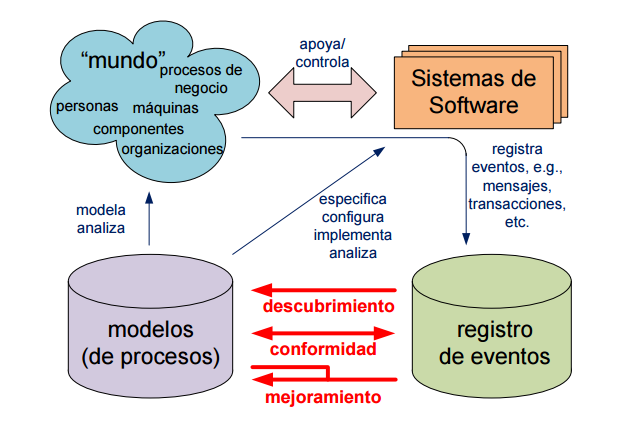
\includegraphics[scale=0.5]{img/pmcycle.png}\\
    \caption{Interacción de los diferentes tipos de PM.}
    \label{fig:pmcycle}
\end{figure}

Al relacionar el comportamiento de un log $\pmlog$, el lenguaje de una red, i.e. $\Language(N)$ y 
el propio sistema $\sys$, se definen nuevos conceptos~\cite{BuijsDA14}
que ayudan a cuantificar la calidad del modelo propuesto: modelo \emph{incompleto},
modelo \emph{adecuado}, modelo \emph{preciso}, modelo \emph{generalizador} de un log y \emph{simpleza} de un modelo.
%incomplete, fitness, precise, generalization, simple

\begin{itemize}
  \item $\pmlog$ se dice incompleto con respecto a un sistema $\sys$ si existen comportamientos
        de $\sys$ no representados en $\pmlog$, i.e. ${\sys} \setminus \pmlog \ne \emptyset$.
  \item $N$ se dice adecuado con respecto a un log $\pmlog$ si el modelo captura el comportamiento 
        de las trazas en $\pmlog$, i.e. $\pmlog \subseteq \Language(N)$.
  \item $N$ se dice preciso con respecto a un log $\pmlog$ si $N$ no admite ejecuciones que no hayan
        sido observados en $\pmlog$, i.e. $\Language(N) \setminus \pmlog = \emptyset$.
  \item $N$ se dice una generalización de un log $\pmlog$ sobre un sistema $\sys$ si $N$
        no se restringe al comportamiento observado en $\pmlog$ y acepta trazas que no han sido observadas aún,
        i.e. $({\sys} \setminus \pmlog) \cap \Language(N) \neq \emptyset$.
  \item $N$ se dice simple cuando posee la menor complejidad posible y representa $\Language(N)$.
        Es ampliamente aceptado que el tamaño de un modelo de procesos constituye el indicador más importante
        sobre la simplicidad del mismo~\cite{AalstBook,Aalst2012,LeonRCHH15,CarmonaC14}.
\end{itemize}

El primero de los enfoques de la minería de procesos, el descubrimiento de procesos, busca extraer un modelo $N$
(e.g. diagrama UML, BPMN, red de Petri) a partir de un log $\pmlog$ con el objetivo de modelar
el proceso subyacente en un cierto sistema $\sys$. 

La validación de procesos, por su parte, comprende analizar la calidad de un cierto modelo,
posiblemente obtenido mediante las técnicas de descubrimiento del punto anterior. En este punto, 
son necesarios, por lo menos, un modelo $N$ y un log $\pmlog$ y consiste en medir la calidad 
de $N$ en reproducir los comportamientos observados en $\pmlog$. Para medir la calidad de $N$ se 
utilizan los conceptos ut supra definidos:
se busca un modelo \emph{adecuado}, \emph{preciso}, \emph{general} y \emph{simple}.

Por último, la mejora de modelos, tiene como objetivo extender y mejorar un modelo dado utilizando la información
del proceso real obtenida a partir de los logs. En este punto, se buscan detectar posibles dificultades en 
el modelo así como también reducir su complejidad.


\section{Redes de Petri}
\label{sec:2.Petrinets}
Las \textbf{redes de Petri}, introducidas en el año 1962 por el matemático
Carl Adam Petri, consisten en una generalización de la teoría de autómatas.
Nacidas de la necesidad de representar sistemas dinámicos con eventos concurrentes;
forman un lenguaje gráfico y matemático con una semántica formal.
Desde su creación han sido utilizadas, entre otros usos, para representación,
análisis, verificación y simulación de sistemas de eventos discretos con 
comportamiento dinámico~\cite{Murata89}.

Una red de Petri está formada por dos componentes, la red propiamente dicha y un conjunto
de \dquote{fichas} asignadas a ciertos nodos de la misma.

La primera de estas componentes consiste en un grafo bipartito dirigido y ponderado,
cuyos nodos se separan en los conjuntos disjuntos 
llamados \textit{places} y transiciones -\textit{transitions}-.
Los arcos del grafo se dirigen tanto de los places a las transiciones como viceversa.

En el momento de graficar una red de Petri, los places, generalmente se
representan mediante círculos y las transiciones mediante cajas o barras.

La segunda componente de una red de Petri consiste en la asignación
de un número entero de fichas o marcas a cada uno de los places, 
utilizado para simular el comportamiento dinámico y concurrente del sistema.
A la distribución de estas marcas sobre cada uno de los places, se la denomina
\textit{marking} y corresponde al estado en el cual se encuentra en cada momento el sistema.
La distribución inicial de estas fichas, por tanto, se conoce como \textit{marking inicial}.

Gráficamente, esta asignación se representa de manera distribuida, indicando dentro 
de cada place el número entero asignado por el marking, o bien, dibujando una 
cantidad de puntos igual a dicho número.

Formalmente, una red de Petri es una 4-upla $(P,T,F,M_0)$ donde $P$ y $T$\footnotemark[1]
representan los conjuntos finitos y disjuntos de places y transiciones respectivamente.
Por su parte, los arcos ponderados vienen dados por \mbox{$F:(P \times T) \cup (T \times P)  \to \nat$}
y un marking $M$ viene dado por la función \mbox{$M:P \to \nat$}.
Por último, $M_0$ representa el estado inicial de la red, i.e. el marking inicial.

\footnotetext[1]{ En este trabajo, utilizamos el mismo símbolo $T$ para denotar el conjunto de transiciones
    de una red de Petri así como para el alfabeto de actividades de las trazas de un log.
    Esta colisión es intencionada ya que, en nuestro modelo, cada transición se corresponde biunívocamente
    con una actividad del log.
}

El \textit{preset} y \textit{postset} de un place $p$ corresponden al conjunto 
de transiciones que \dquote{llegan} y \dquote{salen} de $p$. Se denotan como $\preset{p}$ y $\postset{p}$
respectivamente, los cuales se definen formalmente como: $\preset{p} =  \{t \in T ~|~ F(t,p) > 0 \}$
y $\postset{p} = \{t \in T ~|~ F(p,t) > 0 \}$.

Se le llama red de Petri \emph{pura} a una red que no posee ciclos de longitud uno, i.e.
$\forall p \in P:~ {\preset{p}} \mathrel{\cap} {\postset{p}} = \emptyset$.
En adelante, asumiremos que todas las redes de Petri con las que trabajamos son puras.
Esto es una consecuencia de utilizar la teoría de poliedro como se verá en el siguiente capítulo
\todo[inline]{Ver a que debemos hacer referencia acá. se que en algún lado lo escibí...}.
Es importante destacar que esto no es una 
restricción importante ya que podemos, de manera sistemática, relajar un modelo no puro agregando
places ficticios y convertir cualquier ciclo de longitud uno en un ciclo de longitud dos para
obtener una red de Petri pura.

Como notamos anteriormente, las redes de Petri se utilizan para representar sistemas 
dinámicos; este comportamiento dinámico está definido mediante las \emph{reglas de evolución}.
Intuitivamente, el dinamismo de una red viene dado por los markings que se encuentran en cada
uno des sus places, los cuales se van \dquote{moviendo} de un place a otro a través de la 
ejecución de las transiciones. 
Para que una transición pueda ser recorrida, debe estar \emph{habilitada}. Una transición 
$t \in T$ está habilitada, en un cierto marking $M$ si 

\bequation
    \mbox{$\forall p \in P:~ M(p) \ge F(p,t) $}.
\eequation

Es decir, una transición $t$ se encuentra habilitadas, si el marking contiene suficientes
fichas como marca el preset de $t$.

Ejecutar una transición $t$ sobre un place $p \in P$ en un cierto marking genera 
un nuevo marking $M'$, esto se denota \firing{M}{t}{M'}.
$M'$ viene definido de manera incremental como
\bequation
    M'(p) = M(p) - F(p,t) +  F(t,p)
\eequation

Una cierta secuencia de transiciones \mbox{$\sigma = t_1,t_2, t_3, \ldots, t_n$}
se dice ejecutable si existe una secuencia de markings \mbox{$M_1, M_2, \ldots, M_n$}
tal que pueda suceder la siguiente evolución
\bequation
    \firing {\firing {\firing {\firing {M_0} {t_1} {M_1}} {t_2} {M_2} } {t_3} {\cdots}} {t_n} {M_n}.
\eequation

Dada una red de Petri $N$, se llama $\Language(N)$ al lenguaje de la misma, i.e.
el conjunto de secuencias de transiciones ejecutables sobre $N$.
Por su parte, al conjunto de markings alcanzable partiendo desde el marking inicial $M_0$,
llamado \emph{conjunto alcanzable} de $N$, se lo nota $\rs(N)$.

\begin{figure}[h]
  	\centering
    \begin{tikzpicture}

  \node[transition] (x) at (-.75,-1) {$x$};
  \node[transition] (y) at (.75,-1) {$y$};
  \node[tplace,label=above:$p_1$] (p1) at (0,0) {};
  \node[tplace,label=below:$p_0$] (p2) at (0,-2) {};
      
  \node[] (t) at (p1) {6};
  \node[] (t) at (p2) {1};
    
  \draw[style={->,>=triangle 45}] (p1) edge node[above left]{2} (x);
  \draw[style={->,>=triangle 45}] (x) to (p2);    
  \draw[style={->,>=triangle 45}] (p2) to (y);      
  \draw[style={->,>=triangle 45}] (y) edge node[above right]{3} (p1);
  
  \node[] (null) at (0,-3) {};
  
\end{tikzpicture}

    \caption{Una red de Petri (pura) con pesos no unitarios.}
    \label{fig:pn1}
\end{figure}

Sea $p$ un place con \mbox{$\preset{p}=\{x_1,\ldots,x_k\}$}, \mbox{$\postset{p}=\{y_1,\ldots,y_l\}$} 
y una función de marcado $M$ constante  tal que a cada place le asigna 1 token.
Siendo $M_0(p)$ la cantidad de tokens en el marking inicial 
para el place $p$, entonces, la siguiente ecuación
se satisface para cualquier secuencia $\sigma$

\bequationl{1place_cte}
    M(p) = M_0(p) + \widehat\sigma(x_1)+\cdots +\widehat\sigma(x_k) - \widehat\sigma(y_1)-\cdots -\widehat\sigma(y_l).
\eequation

Generalizando la ecuación \eqref{eq:1place_cte} para permitir arcos ponderados, se tiene

\bequationl{1place_wei}
    M(p) = M_0(p) + \sum_{x_i \in \preset{p}}F(x_i,p)\cdot \widehat\sigma(x_i) - \sum_{y_i\in\postset{p}}F(p,y_i)\cdot\widehat\sigma(y_i).
\eequation

Ahora, si se extiende \eqref{eq:1place_wei} a todos los places de una red de Petri,
utilizando la notación matricial, se obtiene la ecuación conocida como 
\emph{ecuación de marcado} de una red de Petri~\cite{Murata89}

\bequationl{matrix_eq}
    M = M_0 + A \cdot \widehat\sigma,
\eequation

donde $M$ y $M_0$ son vectores y $A$ representa la \emph{matriz de incidencia}
del grafo; La matriz $A$ posee $|P|$ filas y $|T|$ columnas y representa las conexiones 
existentes en la red.

De la ecuación \eqref{eq:matrix_eq} se desprende el concepto
de \textit{conjunto potencialmente alcanzable} el cual corresponde al conjunto
de soluciones de la siguiente inecuación

\bequationl{matrix_ineq}
    M = M_0 + A \cdot \widehat\sigma \geq 0.
\eequation

%Utilizando la ecuación \eqref{eq:matrix_ineq} resulta natural definir el concepto
%de complejidad de una red de Petri como la suma
%de los valores absolutos de todos los coeficientes de la matriz $A$ con la suma
%de los valores absolutos del vector de $M_0$.

A continuación, a modo de ejemplo, se construye la ecuación \eqref{eq:matrix_ineq} de
la red de Petri de la ~\autoref{fig:pn1}, 

\bequation
    \left[\begin{array}{c} 1 \\ 6 \end{array} \right] +
    \left[\begin{array}{rr} 1 & -1 \\ -2 & 3 \end{array} \right]
    \cdot
    \left[\begin{array}{c} \widehat\sigma(x) \\ \widehat\sigma(y) \end{array} \right]
    \geq 
    \left[\begin{array}{c} 0 \\ 0 \end{array} \right].
\eequation

Es importante ver que todo marking alcanzable de una red de Petri
satisface \eqref{eq:matrix_ineq}, sin embargo, lo opuesto no siempre es cierto.
En general, pueden existir markings no alcanzables para
los cuales \eqref{eq:matrix_ineq} se satisface, i.e. $\rs(N) \subseteq \prs(N)$~\cite{SilvaTC96}.

\section{Dominios numéricos abstractos}
\label{sec:2.discovery}

El enfoque presentado en esta tesina utiliza dominios numéricos abstractos sobre los datos provenientes
del log de un cierto sistema para obtener un modelo formal del mismo.
La idea principal consiste en convertir las diferentes trazas de eventos en un conjunto de puntos
en el espacio mediante el uso de los \textit{vectores Parikh} para luego, mediante métodos 
de programación lineal, obtener un poliedro convexo que contenga dichos puntos. 
Luego de obtener este poliedro, se muestra como puede derivarse una red de Petri 
que modela el procesos del sistema.

\subsection{Vectores Parikh} 
\label{sec:2.parikh}

Dada una traza $\sigma=\sigma_1\cdot\sigma_2\cdot\ldots\cdot\sigma_n$, sobre un alfabeto
$T=\{t_1,t_2,\dots,t_n\}$, se utiliza $|\sigma|_{t_i}$ para representar la
cantidad de ocurrencias de $t_i$ en $\sigma$.
Luego, el \emph{vector Parikh} de $\sigma$ se define como un vector
de longitud $n$ en el cual cada componente toma como valor la cantidad de ocurrencias
de la actividad asociado al evento.

\begin{definition}
    \label{def:pv}
    (Vector Parikh). Sea $T=\{t_1,\ldots,t_n\}$ un alfabeto de actividades,
    el vector Parikh de una secuencia de eventos sobre $T$ se define como
    la función

    \bequation
        \begin{array}{lll}
            \widehat{\ }:& T^*&\rightarrow \nat^n\\
            \;&\sigma &\mapsto \widehat{\sigma}=(|\sigma|_{t_1},\dots, |\sigma|_{t_n} ).
            %\widehat{\sigma}&=&(|\sigma|_{t_1},\dots, |\sigma|_{t_n} )
            %\widehat{\sigma}:& \sigma&\mapsto (|\sigma|_{t_1},\dots, |\sigma|_{t_n} )
        \end{array}
    \eequation
Además, por simplicidad, se denota cada $|\sigma|_{t_i}$ como $\widehat\sigma(t_i)$.
\end{definition}

\begin{definition}
    \label{def:pv_log}
    (Vectores Parikh de un log). Dado un log $\pmlog$, el conjuncto de
    vectores Parikh de $\pmlog$ se define como

    \bequation
        \parikh{\pmlog}=\{ \widehat\sigma ~|~ \sigma \in \pmlog \}.
    \eequation

\end{definition}

\begin{example}
    Dadas las trazas  $\sigma_1=t_1 \cdot t_2 \cdot t_1 \cdot t_2 \cdot t_1 \cdot t_1 \cdot t_3$
    y $\sigma_2=t_4 \cdot t_4$ sobre el alfabeto $T=\{t_1,t_2,t_3,t_4\}$,
    se tiene que los vectores Parikh de cada traza son: $\widehat{\sigma_1} = (4,1,1,0)$ y
    $\widehat{\sigma_2} = (0,0,0,2)$ y si se toma \mbox{$\pmlog =\{\sigma_1,\sigma_2\}$}
    se tiene que $\parikh{\pmlog}=\{ (0,0,0,2),(4,1,1,0) \}$.
\end{example}

Dado que los vectores Parikh no consideran el orden de los eventos, la función \mbox{$\widehat{\ }$} no 
es una función inyectiva, i.e. dos trazas diferentes pueden poseer la misma representación como Parikh
vector.
%However since we transform every prefix of a trace into a point,
%there is no loss in expressivity:
%traces $a \cdot b$
%and $b \cdot a$ generate the vector $(1,1)$,
%however the former also generates $(1,0)$ since this is the Parikh vector of its prefix $a$,
% but this vector is not generated by $b \cdot a$.

\subsection{Poliedros convexos y látices enteras} 
\label{sec:2.discovery polyhedra}

Un \textit{semiespacio} es cada
una de las porciones en las que queda dividido un espacio $n$-dimensional por un hiperplano $(n-1)$-dimensional. Un semiespacio
puede ser descripto mediante un incuación lineal de la forma $$a_1x_1 + a_2x_2 + \cdots + a_nx_n \geq b.$$

Un poliedro convexo $n$-dimensional es un conjunto convexo de puntos en $\mathbb{R}^n$. Existen 
dos maneras de representar un poliedro convexo, la $V$-representación y la $H$-representación~\cite{Rockafellar70}.
En este trabajo, se utiliza la segunda, la cual representa un poliedro convexo $\ph$ 
como la intersección de un conjunto de $k$ hiperespacios,

\bequationl{convex_poly}
    \ph = \{ x \in \mathbb{R}^n ~|~ A\cdot x + b \geq 0\}
\eequation
donde  \mbox{$A \in \mathbb{R}^{k \times n}$} y
\mbox{$b\in\mathbb{R}^{k}$}.

En adelante, cuando se habla simplemente de un poliedro se hace referencia a un poliedro convexo,
excepto que se indique lo contrario.
%Los siguientes resultados son importantes para el resto del trabajo~\cite{CarmonaC14}:
%
%\begin{theorem}
%\label{theo:orig_in_b_pos}
%    Sea $\ph$ un poliedro convexo definido como la intersección de un conjunto
%    finito de semiespacios siguiendo \eqref{eq:convex_poly}. $\ph$ contiene el 
%    origen \mbox{$z=(0,\ldots,0)$} sí y solo sí, $b \geq 0$.
%\end{theorem}
%
%\begin{proof}
%    Si el orígen pertenece a $\ph$, entonces $b$ debe tener todas sus componentes positivas,
%    en caso contrario una de las inecuaciones no se cumpliría al evaluar el origen.
%    Por otro lado, si $b \geq 0$, entonces el origen satisface todas las inecuaciones.
%\end{proof}

Se denomina látice entera, y se denota $Z^n$, a una látice en el espacio Euclidiano $\mathbb{R}^n$
cuyos puntos son $n$-uplas de enteros. 
Dado un poliedro convexo $\ph$, el conjunto de puntos enteros dentro de $\ph$
forman una látice entera, denominada $Z$-poliedro de $\ph$.
% Cambió de idioma y se transvistió...
Dado que en este trabajo se utilizará un poliedro convexo que contenga la representación como vectores Parikh
de un log, el espacio estará restringido a pntos entereso, i.e. al $Z$-poliedro correspondiente.

\subsection{Descubrimiento de procesos} 
\label{sec:2.discovery discovery}

El objetivo del \textit{descubrimiento de procesos} es encontrar un 
modelo $N$ (e.g. una red de Petri) que represente, el comportamiento 
observado en un cierto log $\pmlog$.

En~\cite{CarmonaC14} se presentan diferentes técnicas 
para el descubrimiento de redes de Petri a partir del 
conjunto de vectores Parikh de un log $\pmlog$.
En él, se utiliza el conjunto $\parikh{\pmlog}$ para encontrar
la matriz $A$ y el marking inicial $M_0$ de la ecuación \eqref{eq:matrix_ineq};
de esta manera la red de Petri que se obtiene resulta 
una buena aproximación del proceso que genera el log $\pmlog$.

Dada una red de Petri $N$, comparando las expresiones \eqref{eq:matrix_ineq}
y \eqref{eq:convex_poly}, se puede observar que $\prs(N)$ se corresponde con
un $Z$-poliedro de un poliedro convexo que posee dos propiedades:
\mbox{$A \in \mathbb{Z}^{|P|\times|T|}$} y \mbox{$M_0 \in \mathbb{N}^{|P|}$}.
Estas propiedades, son garantizadas por el proceso de construcción ya que el
marking inicial es siempre no negativo y sólo markings con valores enteros positivos
son alcanzables.


La látice entera n-dimensional $\mathbb{Z}^n$ es la látice de las $n$-uplas
de enteros que representan a los elementos de $\parikh{\pmlog}$. Así, un log 
puede representarse como un conjunto de \dquote{caminatas} en $\mathbb{N}^n$. Cada paso 
en una caminata se mueve de un punto de la látice a otro aumentando únicamente uno de
los componentes de la $n$-upla en una unidad.

En \autoref{fig:simp}, se puede ver la correspondencia entre un log y una red
de Petri.  En ~\autoref{sfig:simp.1} se representan tres caminatas en un espacio
bidimensional. Las áreas en gris claro representan un poliedro que contiene todos 
los puntos visitados por las tres caminatas. Dicho poliedro, puede representarse como 
la intersección de dos semiespacios en $\mathbb{R}^2$

\begin{figure}[h]
  \centering
  \subbottom[\label{sfig:simp.1}]{%
    \scaledinput{0.37}{img/ineq}}
  \hfill
  \subbottom[\label{sfig:simp.2}]{%
    \scaledinput{0.9}{img/ineq_net1}}
  \hfill
  \subbottom[\label{sfig:simp.3}]{%
    \scaledinput{0.9}{img/ineq_net2}}
  \caption{Caminatas en la látice entera y red de Petri.}
  \label{fig:simp}
\end{figure}




\bequation
    \begin{array}{lllllll}
        p_0 = 1&+&\widehat\sigma(x)&-&\widehat\sigma(y)&\geq&0\\
        p_1 = 6&-&2\cdot\widehat\sigma(x)&+&3\cdot\widehat\sigma(y)&\geq&0
    \end{array}.
\eequation

El poliedro puede ser representado también, de la forma de la ecuación \eqref{eq:matrix_ineq} 
obteniendo así la interpretación de la ecuación de marcado para la red de Petri en ~\autoref{sfig:simp.2}.
Cada semiespacio del poliedro, i.e. cada fila de la matriz, está representado por un place de la red.
El conjunto de vectores Parikh generados por esta red corresponden al $Z$-poliedro del poliedro 
representado en ~\autoref{sfig:simp.1}.

%En resumen, dado un log $\pmlog$, podemos aplicar las técnicas introducidas en~\cite{CarmonaC14}
%al conjunto $\parikh{\pmlog}$ para obtener un poliedro que pueda luego ser transformado en 
%una red de Petri siguiendo un razonamiento análogo al ejemplificado.

\begin{remark}
    Al haber introducido la relación existente entre semiespacios y places de una red, 
    se puede observar por qué el método utilizado se limita a redes de Petri puras. 

    Si se considera un place $\emph{p}$ el cual se encuentra tanto en el preset como en el postset
    de una transición $\emph{t}$,  la variable que representa a $\emph{t}$ en el semiespacio 
    correspondiente a $\emph{p}$ no podrá capturar el hecho de que la transición
    es producida ($\emph{t}$ con un cierto coeficiente positivo, $\emph{+k}$) 
    y consumida ($\emph{t}$ con un coeficiente negativo, $\emph{-k}$) 
    al mismo tiempo. Esto se debe a que los coeficientes (i.e. $+k,-k$) se cancelan mutuamente.
\end{remark}

\section{Información negativa} 
\label{sec:2.negative}

Existen diferentes interpretaciones para el término \textit{información negativa}. Por ejemplo, en aprendizaje automático,
el término hace referencia a un comportamiento que posee una etiqueta negativa, e.g. para un grupo
de estudiantes de un curso, la información positiva corresponden a aquellos estudiantes que aprueban el curso
y la información negativa, aquellos estudiantes que reprueban el curso. 

En el campo de la minería de procesos, por lo general, la noción utilizada de información negativa es diferente;
una traza negativa corresponde a un comportamiento prohibido, una secuencia de eventos que se desea 
evitar durante la ejecución del sistema y como tal no debe ser aceptado en el modelo.

\begin{definition}
    \label{def:neg}
    (Trazas negativas) Una cierta secuencia $\sigma=\sigma_1\cdot\sigma_2\cdot\ldots\cdot\sigma_n$ es
    una traza negativa (o prohibida) del sistema $\sys$ si $\exists k \in \nat, k \lvertneqq n$ tal que
    el prefijo $\sigma'=\sigma_1\sigma_1\cdot\sigma_2\cdot\ldots\cdot\sigma_k \in \sys$ pero $\sigma \notin \sys$
\end{definition}

    Debido al hecho de que los logs de eventos existentes en la vida real rara vez contienen información negativa, 
en este trabajo se utilizan métodos alternativos de obtener dicha información. En~\cite{Goedertier2009} 
y~\cite{BrouckeWVB14} se presentan métodos eficientes de inducir la llamada \textit{información negativa artificial},
basada en la información positiva. 
%En \cite{Goedertier2009,BrouckeWVB14}  el concepto utilizado es de una traza positiva
%a la cual se las concatena con un único evento negativo.
%Corresponde al caso particular en que para todas las trazas negativas,
%según la definición \autoref{def:neg}, $|\sigma'|=k=n-1$. 
En este trabajo se utiliza la \autoref{def:neg}, una versión más general 
a la utilizada en~\cite{Goedertier2009,BrouckeWVB14} ya que se utilizan sufijos
automáticos sobre las trazas negativas obtenidas del algoritmo 
descrito en~\cite{BrouckeWVB14}.
Esta generalización responde al hecho  de que las trazas negativas 
son tranformadas en puntos negativos y luego estos son utilizados
para restringir el proceso de expansión y/o rotación en pos de mejorar el modelo.
Las trazas de la forma utilizada en \cite{Goedertier2009,BrouckeWVB14} generan
puntos negativos que se encuentran muy cercanos al poliedro generado, reduciendo la aplicabilidad del 
método presentado.


\section{Satisfabilidad módulo teorías}
\label{sec:2.smt}

El problema de satisfacer un conjunto de restricciones posee múltiples aplicaciones
en diferentes áreas, incluyendo verificación de hardware o software, inferencia de 
tipos, análisis estático de programas, generación de casos de prueba o problemas en
teoría de grafos. Todos ellos comparten un componente fundamental, utilizan fórmulas
lógicas para describir los estados y las transformaciones de estados que se suceden
en un cierto modelo.

Los problemas más usuales de satisfabilidad consisten en hacer válida una cierta 
expresión booleana, es decir, satisfabilidad de problemas proposicionales 
o \textit{SAT} (de \textit{Propositional \textbf{SAT}isfability Problem}). Para resolverlos,
se cuenta con los conocidos SAT-solvers~\cite{barrettSMT2009}.
Por otra parte, existen problemas cuya modelización es más natural utilizando lenguajes con
mayor poder de expresión, como la lógica de primer orden o lógicas de mayor orden las cuales
admiten diferentes expresiones como variables no booleanes, funciones y cuantificadores.
Para este tipo de problemas, no bastará con utilizar un SAT-solver pero se cuenta con
otro tipo de herramientas, los llamados resolvedores de satisfabilidad módulo teorías
-\textit{satisfability modulo theories solvers}-, los actualmente populares \textit{SMT-solvers}~\cite{deMoura2009}.

Los \textit{SMT-solvers} permiten determinar la veracidad o falsedad de un cierto modelo
basándose en una teoría de fondo aribitraria que otorga mayor expresividad al lenguaje.
Por ejemplo, la teoría aritmética, nos permite utilizar los símbolos  $+$, $<$, $\leq$ 
así como variables numéricas para representar una fórmula para la cual 
el SMT-solver puede (intentar) determinar su veracidad.
\todo[]{No debería agregar el hecho de que no siempre la solución es la misma ni la óptima?}

\section{Enunciado del problema} 
\label{sec:2.problem}

Dado un log $\pmlogp$ y un conjunto de trazas negativas $\pmlogn$ el objetivo de las técnicas utilizadas
en el desarrollo de la tesina es derivar un modelo $N$ con las siguientes características\\

\begin{itemize}
 \item $N$ es una red de Petri pura ponderada;
 \item $\forall \sigmap \in \pmlogp:~ \sigmap \in \Language(N)$, i.e. el modelo admite todo el comportamiento observado;
 \item $\forall \sigman \in \pmlogn:~ \sigman \notin \Language(N)$, i.e. las trazas prohibidas no son aceptadas;
 \item $N$ es simple.\\
\end{itemize}

Los primers tres items son garantizados por la metodología utilizada
en la construcción de la red, por lo que el desafío consiste en minimizar la complejidad del modelo obtenido.

\section{Resumen del capítulo}
\label{sec:2.resumen}
En este capítulo se hizo una introducción a diferentes temas fundamentales para la comprensión y el desarrollo de este trabajo. 
Se presentaron conceptos cruciales como \textit{redes de Petri}, \textit{minería de procesos},
\textit{SMT-solvers}, \textit{poliedros convexos} y \textit{látices enteras}; se dieron definiciones como la de \textit{Vector Parikh} 
y \textit{vectores Parikh de un log} y se describieron ciertas nociones 
utilizadas como las de \textit{logs}, \textit{información negativa} 
o el concepto  entendido por complejidad de una red de Petri.

En particular, se ejemplificó la relación que existe entre ciertas redes de Petri con una látice entera y 
como utilizar esta relación para generar un primer modelo de un sistema a partir de un cierto log.

Por último, utilizando estos conceptos, se presentó una definición formal del problema a tratar en el desarrollo
 de la presente tesina. 
